\section{问题三的分析与求解}

\instruction{本节占位。问题三：长时间干燥（附录 3 变物性，需运行至 2~3 天）。由 @model 提供公式、@impl 求解（注意总计算量与步长选择）、@paper 排版。}

\subsection{模型的建立}
\instruction{控制方程、边界/初始条件占位（沿用问题二的变物性参数化）。}

\subsection{模型的求解}
\instruction{长时间步进、计算量评估、步长无关性验证占位。}

\subsection{结果与分析}
\instruction{结果表/图由 scripts 生成。result3.xlsx 仅含水分浓度（工作表名 Sheet1、时间步长 60 s，见 AGENTS.md §5）。}

% 表格片段本身已是完整的 table 环境，不再套一层（见 05_q2.tex 的说明）。
\IfFileExists{tab/q3_moist.tex}{%
  % 本文件由 scripts/make_tables.py 自动生成，请勿手工编辑
\begin{table}[htbp]
  \centering
  \caption{药材烘干过程的水分浓度（kg/kg；距离单位：cm）}
  \label{tab:q3-moisture}
  \begin{tabular}{cccccc}
    \toprule
    时间/h & 0 & 0.5 & 1 & 1.5 & 2 \\
    \midrule
    6.0000 & 2.0302 & 1.9695 & 1.7782 & 1.4393 & 0.9434 \\
    12.0000 & 0.6840 & 0.6631 & 0.5998 & 0.4895 & 0.2978 \\
    18.0000 & 0.3265 & 0.3181 & 0.2917 & 0.2421 & 0.0604 \\
    24.0000 & 0.2326 & 0.2277 & 0.2122 & 0.1820 & 0.0214 \\
    30.0000 & 0.1940 & 0.1904 & 0.1789 & 0.1559 & 0.0111 \\
    36.0000 & 0.1725 & 0.1695 & 0.1600 & 0.1410 & 0.0070 \\
    42.0000 & 0.1585 & 0.1559 & 0.1477 & 0.1310 & 0.0049 \\
    46.9964 & 0.1500 & 0.1477 & 0.1402 & 0.1249 & 0.0038 \\
    \bottomrule
  \end{tabular}
\end{table}
%
}{%
  \instruction{表占位：tab/q3\_moist（scripts/make\_tables.py 生成）尚未生成。}
}

\begin{figure}[htbp]
  \centering
  \IfFileExists{figs/fig3-C-profiles.pdf}{%
    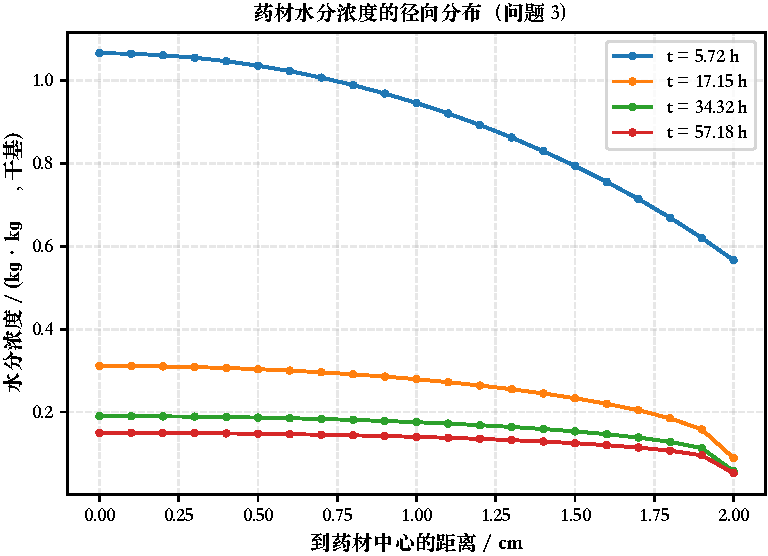
\includegraphics[width=0.75\linewidth]{figs/fig3-C-profiles.pdf}%
  }{%
    \instruction{图占位：figs/fig3-C-profiles.pdf 尚未生成（scripts/make\_figs.py）。}
  }
  \caption{长时间干燥下药材内部水分浓度分布}
  \label{fig:q3-concentration}
\end{figure}
